\documentclass{NoteThesis/note-thesis}

\course{Materials and Sustainability}

\coursetitle{QXU6008 Materials and Sustainability}
\semester{2025B}
\teacher{Prof. Maria Romero-Gonzalez and Prof. Giuseppe Viola}

\begin{document}

\maketitle

\tableofcontents

\newpage

\section{Introduction to Module}

\subsubsection*{Sustainability}

The ability of self maintain over a period of time.

\subsection*{Assessment}

\begin{table}[h]
    \centering
    \begin{tabular}{cc}
        \hline
        Activity & Score\\
        \hline
        Group Coursework & 30\%\\
        -Peer Assessment & 10\%\\
        Individual Coursework & 40\%\\
        Exam in Week10 & 20\%\\ 
        \hline
    \end{tabular}
\end{table}

\section{Sustainable Development Goals}

\begin{itemize}
    \item No Poverty
    \item Zero Hunger
    \item Good Health and Well-being
    \item Quality Education
    \item Gender Equality
    \item Clean Water and Sanitation
    \item Affordable and Clean Energy
    \item Decent Work and Economic Growth
    \item Industry, Innovation and Infrastructure
    \item Reduced Inequalities
    \item Sustainable Cities and Communities
    \item Responsible Consumption and Production
    \item Climate Action
    \item Life Below Water
    \item Life on Land
    \item Peace, Justice and Strong Institutions
    \item Partnerships for the Goals
\end{itemize}

\section{Resource Consumptionb}
\label{resource}

\subsubsection*{Water}

\begin{itemize}
    \item 97\% of water is Salt Water.
    \item 2.2\% of water is Ice.
    \item 0.8\% of water is Fresh Water.
\end{itemize}

Nowaday, in global water consumption, $65\%$ is used for agriculture, and $10\%$ is used for industry.

\subsubsection*{Mineral}

\begin{mynote_env}[frametitle={Mineral Reserve}]
Can be extracted legally and economically using today's technology. Improved extraction technology can enlarge them, but environmental legislation and changing political climate may take them shrink.
\end{mynote_env}

The \textbf{real} total amount of a mineral and it is much larger than the reserve, it is include the current reserve and all other usable deposits that might be revealed by future prospecting.

\subsubsection*{Indicators of Criticality}

\begin{itemize}
    \item The rate of discovery falls below the rate of production
    \item The production rate curve peaks and starts to decline
    \item Materials must be extracted from leaner ore grade
    \item Price fluctuations cease to be intermittent and prices rise permanently
    \item The mineral resource is limited in size or `locked' in one country
    \item The products are economically important or strategically required for national security
\end{itemize}

\begin{figure}[ht]
    \centering
    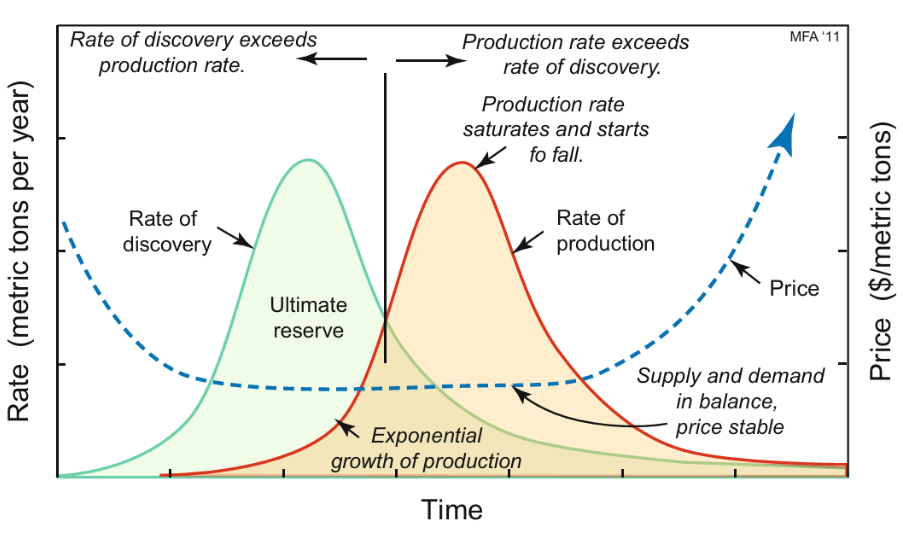
\includegraphics[width=.6\textwidth]{./Figures/Scarcity.png}
    \caption{Predicting Scarcity}
\end{figure}

\section{Business and Sustainability}

\begin{table}[h]
    \centering
    \begin{tabular}{ccccc}
        \hline
        New Tech Capabilities & \multirow{2}{*}{=} & New Ways of Consuming & \multirow{2}{*}{=} & New Business Models\\
        New Social Agendas & ~ & New Ways of Producing & ~ & New Design Approaching \\
        \hline
    \end{tabular}
\end{table}

\subsection{Linear Economy}

Resource Extraction $\to$ Manufacture $\to$ Distribution \& Retail $\to$ Consumer Use $\to$ Disposal

\begin{figure}
    \centering
    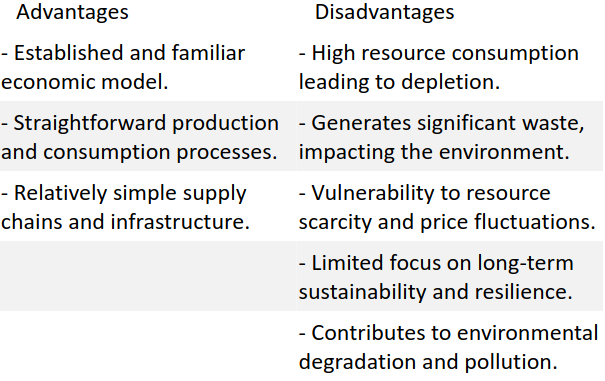
\includegraphics[width=.6\textwidth]{./Figures/Linear_Eco.png}
    \caption{Linear Economy}
\end{figure}

\subsection{Collaborative Economy}

An economy built on distributed networks of connected individuals and communities versus centralized institutions, transforming how we can produce, consume, finance and learn.

\subsubsection*{Different funding models:}
\begin{itemize}
    \item \textbf{Reward-Based:} Funders receive non-financial incentives or rewards.
    \item \textbf{Equity-Based:} Funders receive equities or shares in the project or company.
    \item \textbf{Debt-Based (Crowdlending):} Funders lend money with repayment expectation with interest.
    \item \textbf{Donation-Based:} Funders do not expect financial returns.
\end{itemize}

\subsection{Upstream Innovation}

The early stage of value chain, including design, material selection, and manufacturing process, shipping, and intended use.

For example, eliminate plastic films on cans and bottles, or replace plastic films on vegetables and fruits by eat-able coatings.

\section{Socially Led Approaches to Sustainability}

\subsubsection*{Why Choose Social Approaches}

\begin{enumerate}
    \item Without social social adoption, environmental solutions fail.
    \item Increase long-term impact.
    \item Social justice is important to sustainability.
    \item Trust and local knowledge are important to sustainability.
\end{enumerate}

Three pillars of socially sustainability: \textbf{Equity}, \textbf{Wellbeing} and \textbf{Participation}.

\subsubsection*{Challengs and Limitations}

\begin{itemize}
    \item Unequal participation.
    \item Resource constraints.
    \item Slow decision-making.
    \item Volunteer burnout.
\end{itemize}

\section{Assessing Sustainable Development}

\subsection{System Based}

\subsubsection*{Key Question of Assessing}

\begin{enumerate}
    \item What is it for?
    \item Who wants it?
    \item Who made it?
    \item How did it get there?
    \item What is its impact?
\end{enumerate}

\subsection{Environmentally Led}

\subsubsection*{Eco-Efficieny}

Make technology and production processes cleaner and more efficient through design and innovation.

\begin{enumerate}
    \item Easy to quantifiable;
    \item No significant change to the exiting system;
\end{enumerate}

\subsubsection*{Industrial Symbiosis}

Companies in a region collaborate to utilize each other's by-products and waste materials, creating a more efficient and sustainable industrial ecosystem.

\begin{mynote_env}[frametitle={Biomimicry}]
    Learn how ecosystems manage materials, energy, and how they maintain balance.
\end{mynote_env}

\subsubsection*{Biofabrication}

A new trend in manufacturing, using living organisms or their components to produce materials, chemicals, and products in a more sustainable way.

\subsection{Functional Unit and Declared Unit}

\begin{itemize}
    \item \textbf{Functional Unit:} Represents what the product does or the service it provides, like \textit{Providing user the ability to carry 1L water per day for one year}.
    \item \textbf{Declared Unit:} A specific amount or volume used as the reference unit for comparison, like \textit{A 1L water bottle}.
\end{itemize}

\section{Life Cycle Analysis}

\subsection{Types, or Boundaries}

\begin{itemize}
    \item \textbf{Cradle to Grave}. Includes all stages from raw material extraction to disposal.
    \item \textbf{Cradle to Gate}. Includes stages from raw material extraction to the factory gate (before distribution and use).
    \item \textbf{Gate to Gate}. Includes only the manufacturing process within the factory.
    \item \textbf{Cradle to Cradle}. Focuses on designing products for a circular economy, where materials can be reused or recycled indefinitely.
\end{itemize}

\begin{mynote_env}[frametitle={Eco-Audit}]
    A fast, simplified life-cycle assessment tool used to estimate a product's energy usage and CO$_2$ footprint across its life stages, helping designers quickly compare material and process choices early in the design phase.
\end{mynote_env}

\subsubsection*{Bill of Material}

Also name BOM, a comprehensive list of raw materials, components, and assemblies required to construct, manufacture, or repair a product or service.

\subsection{Life Cycle Impact Assessment}

This phase is to translate the inventory data into environmental impact datas, like \textbf{Carbon Footprint(CO$_{\text{e}}$)}, \textbf{Cumulative Energy Demand(CED)}, \textbf{ReCiPi indicators of the life cycle impact assessment}, or \textbf{Eco-cost}.

\begin{mynote_env}[frametitle={Okala Impact Factor}]
    Created to combine 10 environmental impact categories into a single score, which can be used to compare the overall sustainability of different products or services.
\end{mynote_env}

\section{Material Circularity Indicator}

Track the flow of materials through the economy and assess how well they are being reused, recycled, or repurposed.

The \textbf{Material Circularity Indicator} (MCI) measures the circularity of a product by quantifying how much of its material flow is linear (from virgin feedstock to unrecoverable waste) versus circular (recycled, reused, or sustained).

\subsection{Interpretation of MCI}

\begin{itemize}
    \item \textbf{MCI = 0}: A fully linear product.
    It is manufactured entirely from virgin feedstock and ends up in landfill at the end of its life.
    \item \textbf{MCI = 1}: A fully circular product.
    It contains no virgin feedstock, is completely collected for recycling or component reuse, and the recycling efficiency is 100\%.
    \item In practice, most products fall between these two extremes.
\end{itemize}

\subsection{Five-Step Calculation Procedure}

\subsubsection{Step 1: Virgin Feedstock $V$}

The virgin feedstock is the mass of the product that comes from non-circular sources:
\[
    V = M \times (1 - FR - FU - FS)
\]
where:
\begin{itemize}
    \item $M$: total mass of the product;
    \item $FR$: fraction of feedstock derived from recycled sources;
    \item $FU$: fraction of feedstock derived from reused sources;
    \item $FS$: fraction of biological materials originating from sustained production.
\end{itemize}

\subsubsection{Step 2: Unrecoverable Waste $W$}

The total unrecoverable waste is calculated as:
\[
    W = W_0 + \frac{W_F + W_C}{2}
\]

\paragraph{Direct disposal waste $W_0$.}
This is the mass that is neither recycled, reused, composted, nor used for energy recovery:
\[
    W_0 = M \times (1 - CR - CU - CC - CE)
\]
where:
\begin{itemize}
    \item $CR$: fraction of the product collected for recycling;
    \item $CU$: fraction of the product going into component reuse;
    \item $CC$: fraction of uncontaminated biological materials being composted;
    \item $CE$: fraction of the product used for energy recovery.
\end{itemize}

\paragraph{Waste from recycling the product $W_C$.}
This measures the waste generated when the old product is sent to recycling:
\[
    W_C = M \times (1 - EC) \times CR
\]
where $EC$ is the efficiency of the recycling process used at the end of the use phase.

\paragraph{Waste from producing recycled feedstock $W_F$.}
This measures the waste generated upstream to produce the recycled material used in the new product:
\[
    W_F = M \times (1 - EF) \times \frac{FR}{EF}
\]
where $EF$ is the efficiency of the recycling process used to produce the recycled feedstock.

\paragraph{Why use $(W_F + W_C)/2$?}
The same recycling process connects an old product (which becomes waste $W_C$) and a new product (which uses recycled feedstock, producing waste $W_F$).
Adding $W_F$ and $W_C$ directly would double-count the same recycling losses.
Therefore, half of the total waste is assigned to each product.

\subsubsection{Step 3: Linear Flow Index (LFI)}

The LFI measures the proportion of material flowing in a linear way:
\[
    LFI = \frac{V + W}{2M - \frac{W_C}{2} + \frac{W_F}{2}}
\]
\begin{itemize}
    \item $LFI = 1$: completely linear flow;
    \item $LFI = 0$: completely restorative flow.
\end{itemize}

\subsubsection{Step 4: Utility Factor $X$}

The utility factor accounts for how long and how intensively the product is used:
\[
    X = \frac{L}{L_{AV}} \times \frac{U}{U_{AV}}
\]
where:
\begin{itemize}
    \item $L$: product lifetime;
    \item $L_{AV}$: industry-average lifetime;
    \item $U$: number of functional units delivered over the product lifetime (e.g., wash cycles, km driven);
    \item $U_{AV}$: industry-average use intensity.
\end{itemize}

A longer lifetime or higher use intensity increases $X$, which in turn increases the MCI.

\subsubsection{Step 5: Material Circularity Indicator}

The MCI combines the linear flow index with the utility factor:
\[
    MCI_P = 1 - \left[ LFI \times F(X) \right]
\]

The utility function is defined as:
\[
    F(X) = \frac{0.9}{X}
\]

Therefore:
\[
    MCI_P = 1 - \left( LFI \times \frac{0.9}{X} \right)
\]

To avoid negative values, the final MCI is capped at zero:
\[
    MCI_P = \max(0,\ 1 - [LFI \times F(X)])
\]

\subsection{Worked Examples}

\subsubsection{Example 1: Single-Material, Single-Component Steel Bracket}

Given: $M = 1\ \text{kg}$, $FR = 0.4$, $CR = 0.9$, $EC = EF = 0.7$, $X = 1$.

\begin{table}[h]
    \centering
    \begin{tabular}{lll}
        \hline
        Quantity & Calculation & Result \\
        \hline
        $V$ & $1 \times (1 - 0.4)$ & $0.6\ \text{kg}$ \\
        $W_C$ & $1 \times (1 - 0.7) \times 0.9$ & $0.27\ \text{kg}$ \\
        $W_F$ & $1 \times (1 - 0.7) \times (0.4 / 0.7)$ & $0.171\ \text{kg}$ \\
        $W_0$ & $1 \times (1 - 0.9)$ & $0.1\ \text{kg}$ \\
        $W$ & $0.1 + (0.171 + 0.27)/2$ & $0.321\ \text{kg}$ \\
        $LFI$ & $(0.6 + 0.321) / (2 - 0.135 + 0.086)$ & $0.472$ \\
        $MCI$ & $1 - (0.472 \times 0.9)$ & $\mathbf{0.575}$ \\
        \hline
    \end{tabular}
\end{table}

\subsubsection{Example 2: Single-Material, Multi-Component Steel Product}

Given:
\begin{itemize}
    \item Part A: $M_A = 0.6\ \text{kg}$, $FR_A = 0.5$, $EC = EF = 0.7$;
    \item Part B: $M_B = 0.4\ \text{kg}$, $FR_B = 0.3$, $EC = EF = 0.7$;
    \item $CR = 0.85$, $X = 1$.
\end{itemize}

\textbf{Virgin feedstock:}
\[
    V_A = 0.6 \times (1 - 0.5) = 0.3\ \text{kg}
\]
\[
    V_B = 0.4 \times (1 - 0.3) = 0.28\ \text{kg}
\]
\[
    V = 0.58\ \text{kg}
\]

\textbf{Recycling waste:}
\[
    W_C = 1.0 \times (1 - 0.7) \times 0.85 = 0.255\ \text{kg}
\]

\textbf{Recycled feedstock waste:}
\[
    W_{F,A} = 0.6 \times 0.3 \times \frac{0.5}{0.7} = 0.1286\ \text{kg}
\]
\[
    W_{F,B} = 0.4 \times 0.3 \times \frac{0.3}{0.7} = 0.0514\ \text{kg}
\]
\[
    W_F = 0.18\ \text{kg}
\]

\textbf{Total waste:}
\[
    W = 0.15 + \frac{0.18 + 0.255}{2} = 0.3675\ \text{kg}
\]

\textbf{LFI and MCI:}
\[
    LFI = \frac{0.58 + 0.3675}{2.0 - 0.1275 + 0.09} = 0.483
\]
\[
    MCI = 1 - (0.483 \times 0.9) = \mathbf{0.5653}
\]

\subsubsection{Example 3: Multi-Material, Multi-Component Product}

Given:
\begin{itemize}
    \item Steel bracket: $M = 0.8\ \text{kg}$, $FR = 0.4$, $EC = EF = 0.7$;
    \item Plastic handle: $M = 0.2\ \text{kg}$, $FR = 0.1$, $EC = EF = 0.6$;
    \item $CR = 0.85$, $X = 1$.
\end{itemize}

\textbf{Virgin feedstock:}
\[
    V_{\text{steel}} = 0.8 \times (1 - 0.4) = 0.48\ \text{kg}
\]
\[
    V_{\text{plastic}} = 0.2 \times (1 - 0.1) = 0.18\ \text{kg}
\]
\[
    V = 0.66\ \text{kg}
\]

\textbf{Recycling waste:}
\[
    W_{C,\text{steel}} = 0.8 \times 0.3 \times 0.85 = 0.204\ \text{kg}
\]
\[
    W_{C,\text{plastic}} = 0.2 \times 0.4 \times 0.85 = 0.068\ \text{kg}
\]
\[
    W_C = 0.272\ \text{kg}
\]

\textbf{Recycled feedstock waste:}
\[
    W_{F,\text{steel}} = 0.8 \times 0.3 \times \frac{0.4}{0.7} = 0.137\ \text{kg}
\]
\[
    W_{F,\text{plastic}} = 0.2 \times 0.4 \times \frac{0.1}{0.6} = 0.0133\ \text{kg}
\]
\[
    W_F = 0.1503\ \text{kg}
\]

\textbf{Total waste:}
\[
    W = 0.15 + \frac{0.272 + 0.1503}{2} = 0.36115\ \text{kg}
\]

\textbf{LFI and MCI:}
\[
    LFI = \frac{0.66 + 0.36115}{2.0 - 0.136 + 0.07515} = 0.5266
\]
\[
    MCI = 1 - (0.5266 \times 0.9) = \mathbf{0.5261}
\]

\subsection{Data Sources for Real Products}

\begin{table}[h]
    \centering
    \begin{tabular}{p{2.5cm}p{5cm}p{5.5cm}}
        \hline
        Variable & Meaning & Typical Data Source \\
        \hline
        $M$ & Total product mass & Internal company data (BOM, CAD models, weighing) \\
        $FR$, $FU$, $FS$ & Recycled, reused, and sustained fractions & Supply-chain records and design specifications \\
        $CR$, $CU$, $CC$, $CE$ & Collection fractions for recycling, reuse, composting, and energy recovery & External databases and statistics (e.g., Eurostat, national agencies) \\
        $EC$, $EF$ & Recycling process efficiencies & LCA databases (e.g., Ecoinvent, GaBi) and technical literature \\
        $L$, $U$ & Product lifetime and use intensity & Internal testing or industry surveys \\
        $L_{AV}$, $U_{AV}$ & Industry-average lifetime and use intensity & Market research, academic literature, and national statistics \\
        \hline
    \end{tabular}
\end{table}

\subsection{Applications of MCI}

\begin{itemize}
    \item \textbf{Product design:} informing material selection and design for circularity.
    \item \textbf{Performance reporting:} tracking internal circular-economy progress.
    \item \textbf{Procurement:} comparing circularity scores of different products or suppliers.
    \item \textbf{Portfolio assessment:} aggregating MCI values to product-portfolio or company level.
\end{itemize}

\section{Risk Management and Legislation in Sustainable Development}

\subsection{Resource Limitation}

Most part of this section is mentioned before(\ref{resource})

\subsubsection*{Herfindahl-Hirschman Index}

How much a nation control one resource, the lower index implies less risk to supply chain access and price.

\[
HHI=s_1^2+s_2^2+\cdots + s_n^2
\]

\subsection{Reduce Dependency on Specific Materials}

\begin{enumerate}
    \item \textbf{Short term fluctuations in price.} build reserves or negotiate long-term contracts
    \item \textbf{Long-term supply constraints or Price inflation.} Find substitute materials or re-use.
    \item \textbf{Legislation}.
\end{enumerate}

\section{Ethic in Sustainablity}

Read the QMUL and NPU values.

\end{document}
